\documentclass{article}
\usepackage{graphicx}
\usepackage[utf8]{inputenc}
\usepackage[T1]{fontenc}
\usepackage{graphicx}
\graphicspath{\Slike}
\usepackage{float}
\usepackage{url}
\def\UrlBreaks{\do\/\do-\do\&\do.\do:}

\title{Konfiguracija gaming računala}
\author{Paolo Toth}

\begin{document}

\maketitle

\section{Komponente računala}

\begin{figure}[H]
\subsection{Procesor}
\centering
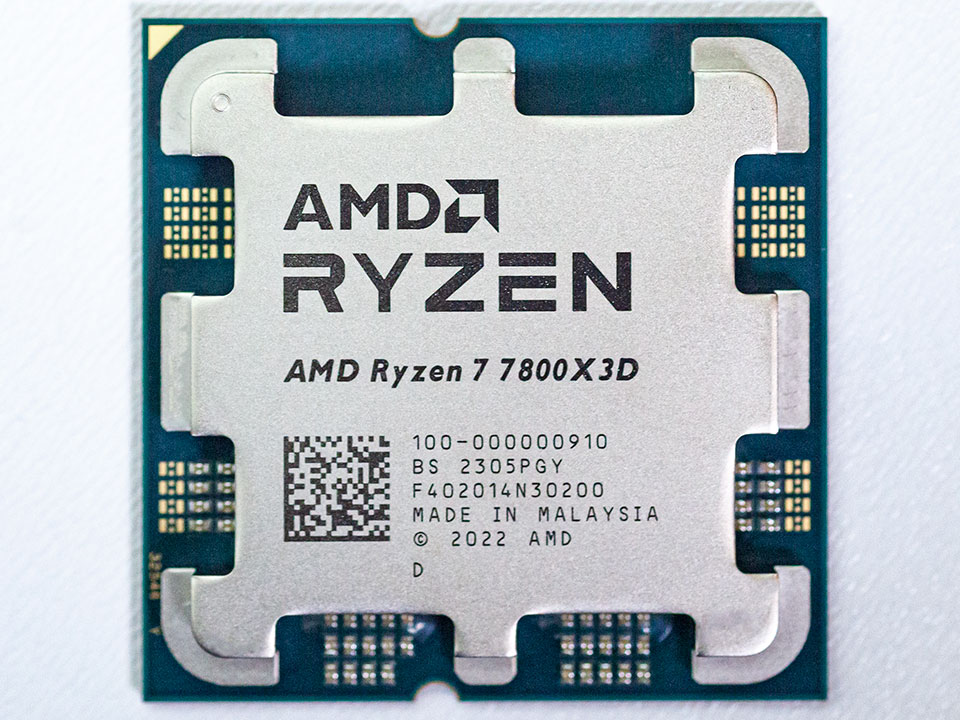
\includegraphics[scale=0.1]{Slike/cpu-front.jpg}
\caption{Ryzen 7 7800X3D AM5, 4.2 GHz, 8 jezgri, 120W TDP} 
Odabrao sam ovaj procesor zbog efikasnosti kod procesa koji koriste sve jezgre, dodatnog L3 cache-a koji pomaže s brzinom dohvaćanja instrukcija što diže framerate u pojedinim igrama. Ovaj procesor teško dostiže svoje termalno ograničenje od 89 stupnjeva i kada je hlađen zrakom.
\end{figure}

\begin{figure}[H]
\subsection{Grafička kartica}
\centering
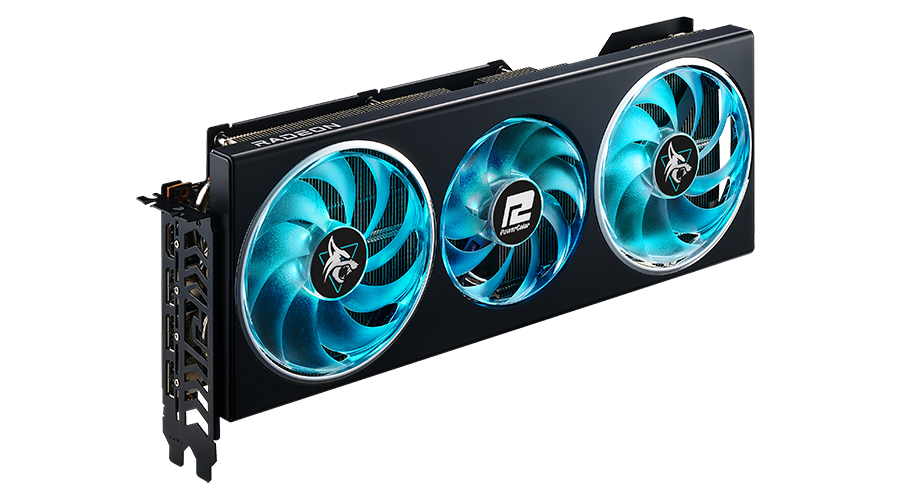
\includegraphics[scale=0.6]{Slike/2307271152084.png}
\caption{Powercolor RX7800XT Hellhound 16GB GDDR6, 2425MHz}
Ova grafička kartica ima 16 GB memorije, jeftinija je i energetski efikasnija od kartica sličnih cijena. Ovo je trenutno najbolja opcija za gaming u 1440p rezoluciji
\end{figure}

\begin{figure}[H]
\subsection{Matična ploča}
\centering
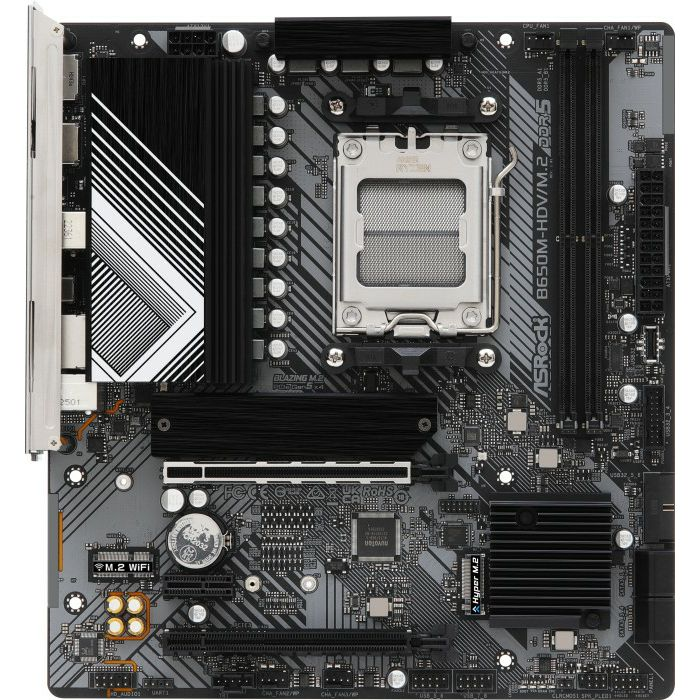
\includegraphics[scale=0.2]{Slike/slika1.jpg}
\caption{Asrock B650M-HDV/M.2}
Ovo je jeftina matična ploča koja ima sva svojstva koja imaju skuplje ploče, osim external clock generatora koji podiže preformanse. Razlika u cijeni između ove i skupljih ploča je neisplativa.
\end{figure}

\begin{figure}[H]
\subsection{RAM}
\centering
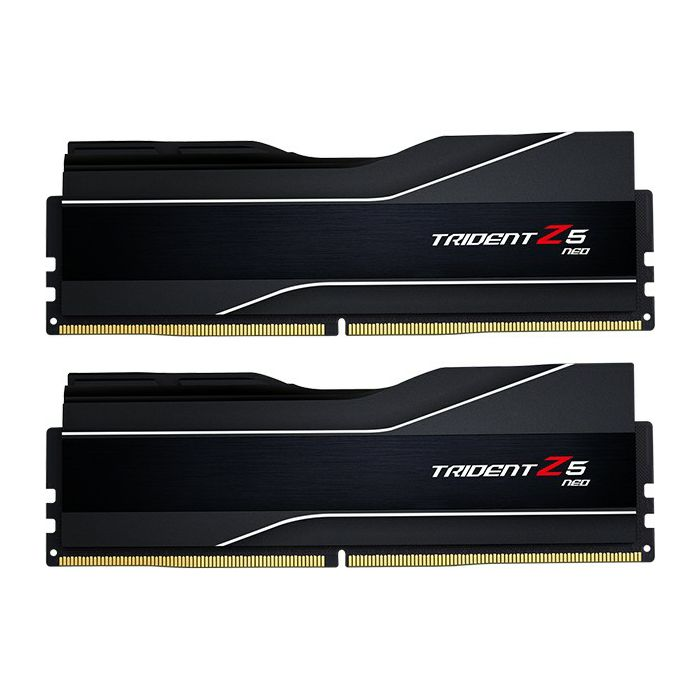
\includegraphics[scale=0.2]{Slike/ram.jpg}
\caption{32 GB G.Skill Trident Z5 NEO Black DDR5, CL30, 6000 MHz}
Ovo je kvalitetan CL30 ram kojem je takt 6000 MHz što je granica stabilnosti za Ryzen procesore. 32 Gb rama polako postaje standard za igranje novih igara zbog njihove veličine i neoptimiziranosti.
\end{figure}

\begin{figure}[H]
\subsection{Pohrana podataka}
\centering
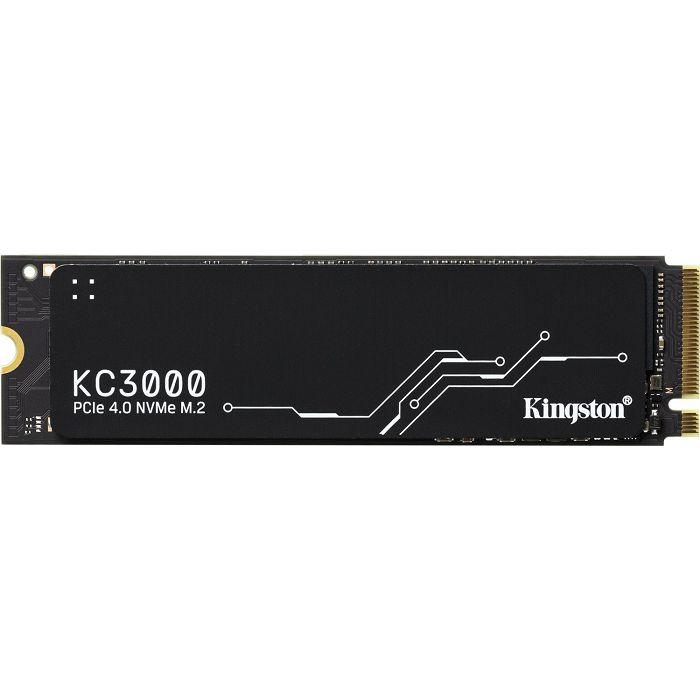
\includegraphics[scale=0.2]{Slike/098700228_55873-2678.jpg}
\caption{Kingston KC3000 M.2, 2TB, NVMe, PCIe 4.0}
Brz i jeftin M.2, osobno koristim ovaj M.2 u dva računala.
\end{figure}

\begin{figure}[H]
\subsection{Napajanje}
\centering
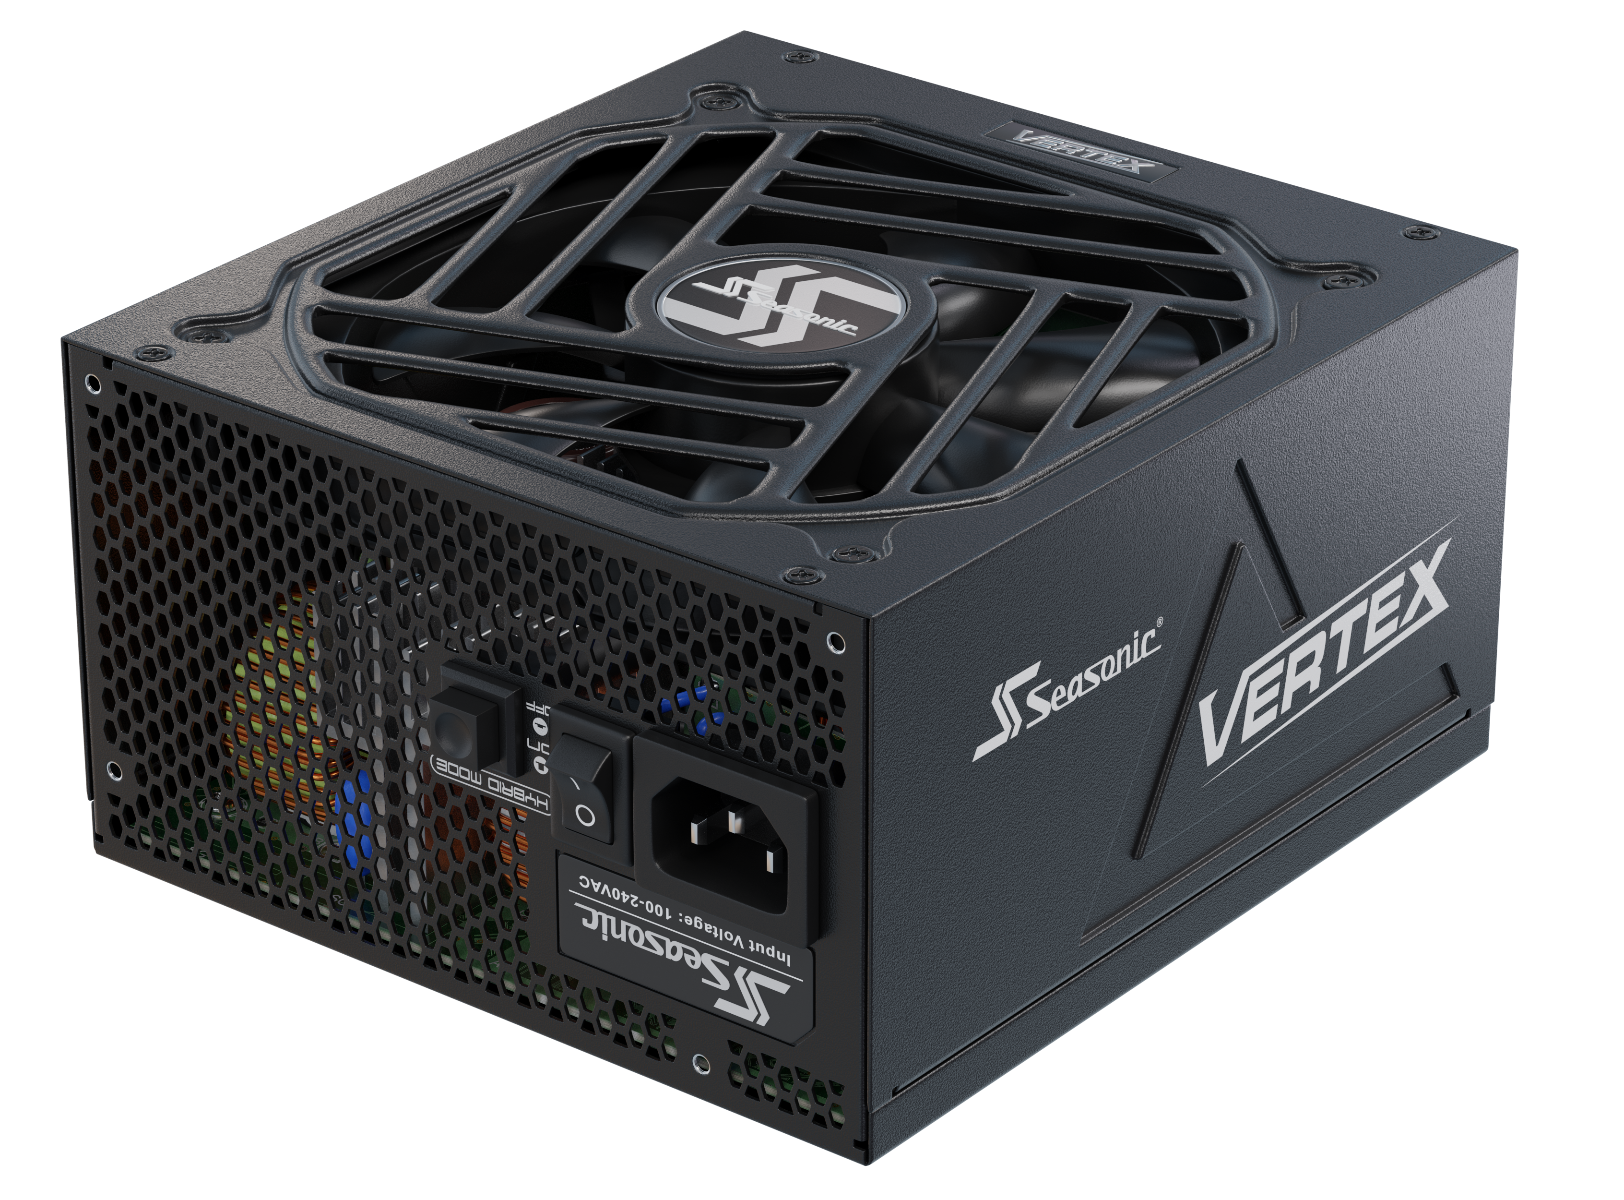
\includegraphics[scale=0.1]{Slike/ver.png}
\caption{Seasonic 1200W VERTEX GX-1200, Full modular, 80 PLUS Gold}
Modularno napajanje s 80 PLUS Gold i Cybenetics Platinum certifikatom. PcPartPicker procjenjuje 534W potrošnje struje, biram ovo napajanje da ne bude preopterećeno i jer ima dva dobra certifikata uz 10 godina garancije.
\end{figure}

\begin{figure}[H]
\subsection{Hladnjak procesora}
\centering
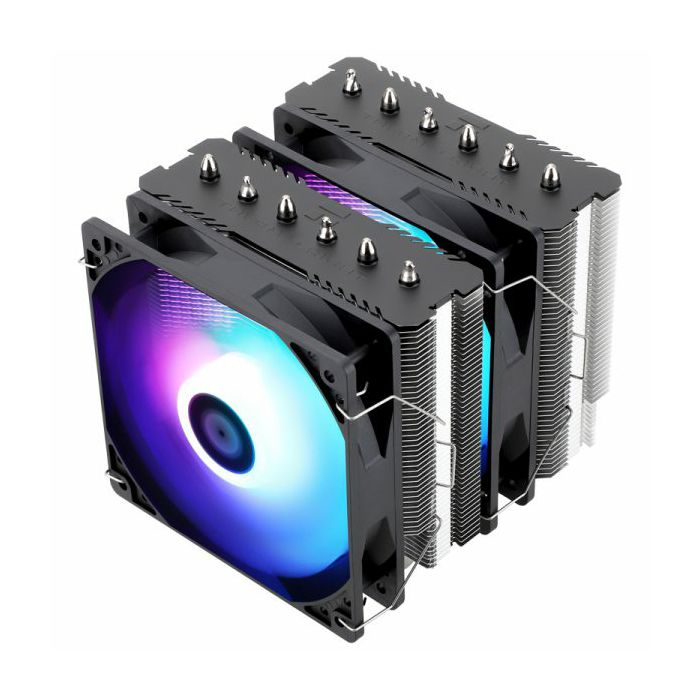
\includegraphics[scale=0.2]{Slike/hl.jpg}
\caption{Thermalright Peerless Assassin 120 SE, 1550 RPM}
Hladnjak podržava AM5, cijena mu nije previsoka i pokazao se odličan na recenzijama.
\end{figure}

\begin{figure}[H]
\subsection{Kućište}
\centering
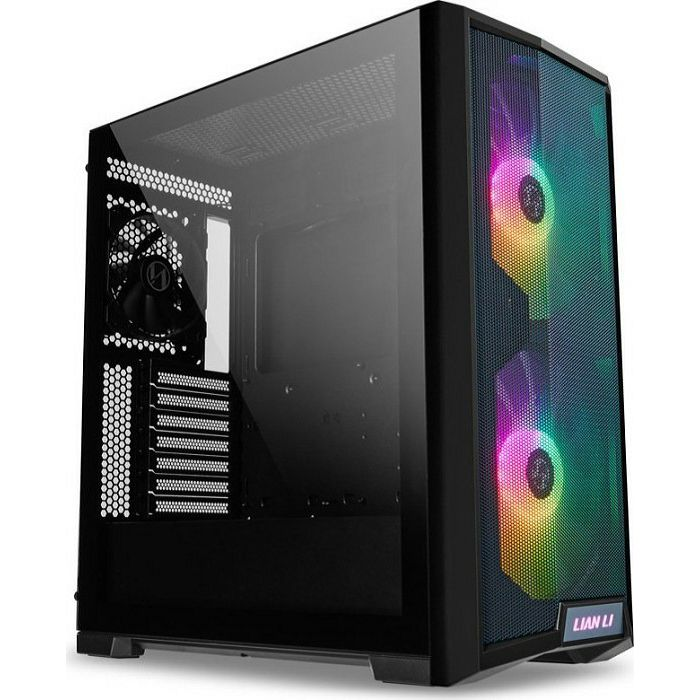
\includegraphics[scale=0.2]{Slike/lan.jpg}
\caption{Lian Li LANCOOL 215}
Odabrao sam ovo kućište jer je dizajnirano za što veći protok zraka, ima dva velika fena of 200mm naprijed tako da je kućište tiho i hladno.
\end{figure}

\section{Periferija}

\begin{figure}[H]
\subsection{Monitor}
\centering
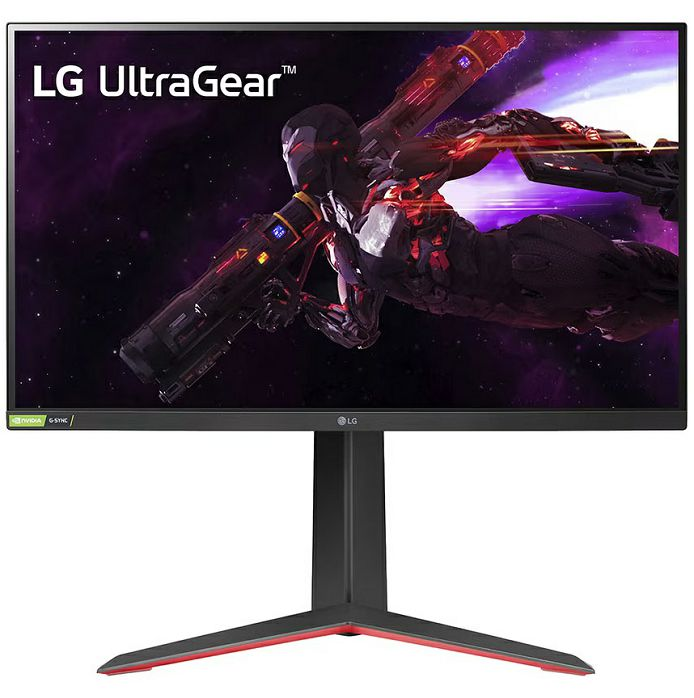
\includegraphics[scale=0.3]{Slike/mon.jpg}
\caption{LG 27" 27GP850P-B, IPS, AMD FreeSync, NVIDIA G-Sync, 165Hz, 1ms, HDR400}
27 inčni monitor koji ima odlično vrijeme odaziva, kvaliteta slike je također dobra.
\end{figure}

\begin{figure}[H]
\subsection{Miš}
\centering
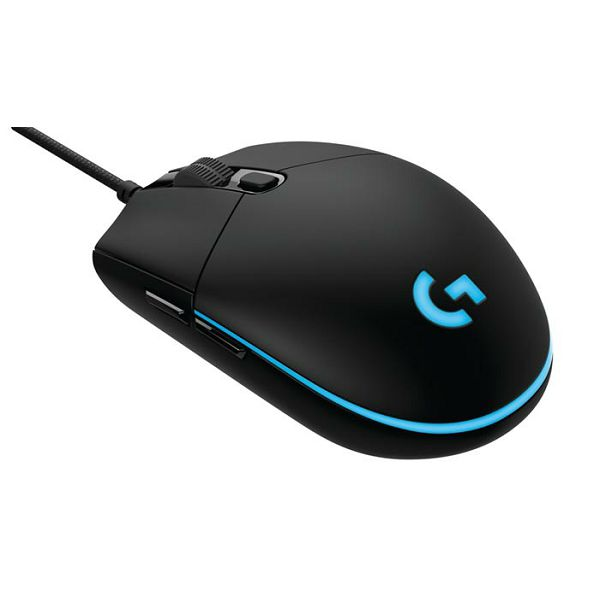
\includegraphics[scale=0.2]{Slike/m.jpg}
\caption{Logitech G Pro Hero, 16000 DPI}
Miš koji koristi najnapredniji Logitechov Hero senzor, odličan miš za cijenu od 50 eura.
\end{figure}

\begin{figure}[H]
\subsection{Tipkovnica}
\centering
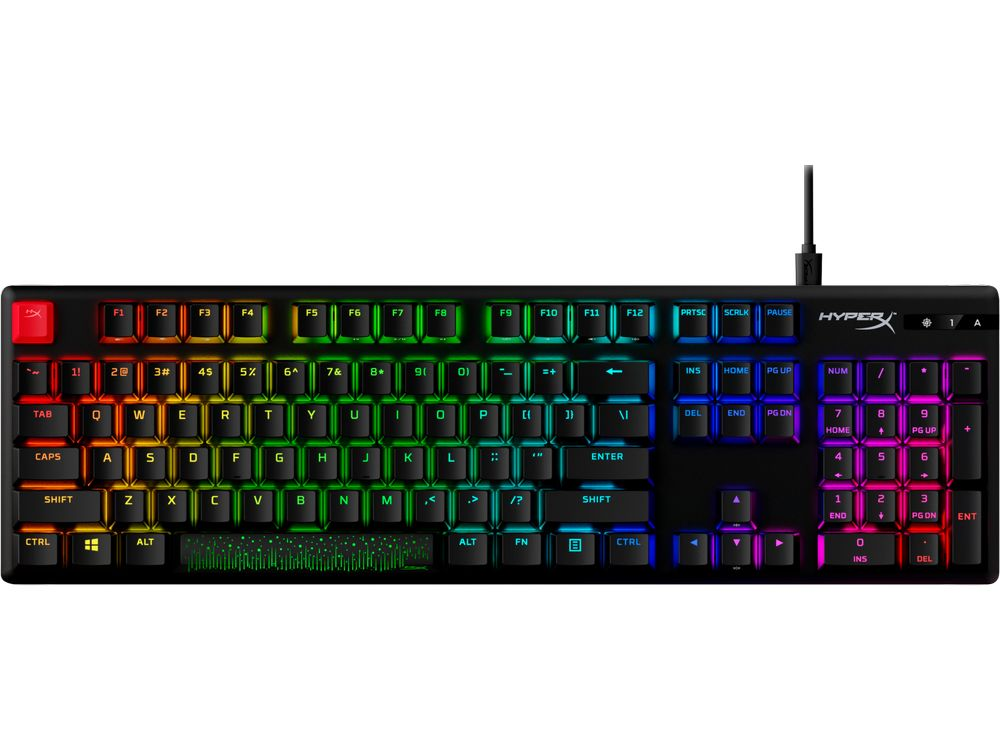
\includegraphics[scale=0.3]{Slike/k.jpg}
\caption{Tipkovnica HyperX Alloy Origins, HyperX Red switch}
Kvalitetna mehanička tipkovnica s linearnim prekidačima.
\end{figure}

\section{Cijena računala}
\begin{itemize}
    \item CPU: AMD Ryzen 7 7800X3D - 477,89 €
    \item GPU: Powercolor RX7800XT Hellhound - 689,47 €
    \item Matična ploča: Asrock B650M-HDV/M.2 - 134,20 €
    \item RAM: G.Skill Trident Z5 NEO Black - 294,74 €
    \item Pohrana podataka: Kingston KC3000 - 189,47 €
    \item Napajanje: Seasonic Vertex GX 1200W 314,74 €
    \item Hladnjak procesora: Thermalright peerless assassin 120 SE 69,00 €
    \item Kućište: Lian Li LANCOOL 215 - 114,74 €
    \item Monitor: LG 27GP850P-B 379,00 €
    \item Miš: Logitech G Pro Hero - 50,53 €
    \item Tipkovnica: HyperX Alloy Origins - 119,99 €
    \newline 
    \newline Ukupna cijena: 2.834,04 €
\end{itemize}

\section{Poveznice}

\begin{itemize}
    \item https://www.adm.hr/powercolor-rx7800xt-hellhound-16gb-rx7800xt-16g-loc/78465/product/
    
    \item https://www.adm.hr/cpu-amd-ryzen-7-7800x3d-box-bez-coolera-420-500ghz-am5-100-100000910wof/77242/product/?utm\_source=nabava.net\&utm\_campaign=nabava.net\-\&utm\_medium=click
    
    \item https://www.adm.hr/asrock-b650m-hdvm2-amd-b650-am5-ddr5-90-mxbla0-a0uayz/78318/product/

    \item https://www.adm.hr/ddr5-32gb-2x16-gskill-6000mhz-trident-z5-neo-black-cl30-f5-6000j3038f16gx/75780/product/

    \item https://www.adm.hr/kingston-ssd-2000gb-kc3000-m2-2280-nvme-pcie-40-skc3000d2048g/75902/product/

    \item https://www.adm.hr/napajanje-seasonic-1200w-vertex-gx-1200-80-gold-vertex-gx-1200/77184/product/

    \item https://www.racunala.hr/thermalright-peerless-assassin-120-se-argb-black/325143/product/

    \item https://www.adm.hr/lian-li-midi-tower-lancool-215-argb-glass-window-black-4718466009654/77475/product/

    \item https://www.instar-informatika.hr/monitor-lg-27-27gp850p-b-nano-ips-gaming-amd-freesync-premium-nv/159251/product/

    \item https://www.adm.hr/logitech-g-pro-hero-zicni-mis/58742/product/

    \item https://www.links.hr/hr/tipkovnica-hyperx-alloy-origins-pbt-mehanicka-hyperx-red-switch-us-cro-layout-crna-usb-010701138?utm\_source=nabava.net\&utm\_campaign\-=nabava.net\&utm\_medium=click

    
\end{itemize}

\section{Izvori informacija}
GPU - https://www.powercolor.com/product?id=1689752075
\newline CPU - https://www.amd.com/en/products/apu/amd-ryzen-7-7800x3d
\newline RAM - https://www.gskill.com/product/165/393/1661410171/F5-6000J3038F16GX2-TZ5N
\newline Matična ploča - https://www.asrock.com/mb/AMD/B650M-HDVM.2/index.asp
\newline Pohrana podataka: https://www.kingston.com/en/ssd/kc3000-nvme-m2-solid-state-drive
\newline Napajanje: https://seasonic.com/vertex-gx
\newline Hladnjak procesora: https://www.thermalright.com/product/peerless-assassin-120-se/
\newline Kućište: https://lian-li.com/product/lancool-215/
\newline Monitor: https://www.lg.com/hr/monitori/lg-27gp850p-b
\newline Miš: https://www.logitechg.com/en-eu/products/gaming-mice/pro-hero.html
\newline Tipkovnica: https://hyperx.com/products/hyperx-alloy-origins-mechanical-gaming-keyboard
\end{document}
